\chapter{Testdokumentation}\label{ch:testdokumentation}
Im folgenden Testfälle mit welchem das Programm getestet wurde.

\definecolor{fhfarbe}{HTML}{00605E}


\section{Vordefinierte Tests}\label{sec:definierte_tests}


% \begin{tabular}{|c|c|c|c|c|c|}
%     \hline
%     a & b & c & U & F & Art \\
%     \hline
%     5 & 3 & 4 & 12 & 6,00 & r, s \\
%     \hline
%     11 & 11 & 10 & 32 & 48,990 & nr, gsch \\
%     \hline
%     29 & 29 & 29 & 87 & 364,164 & nr, gs \\

%     \hline
% \end{tabular}

\begin{figure}
    \centering
    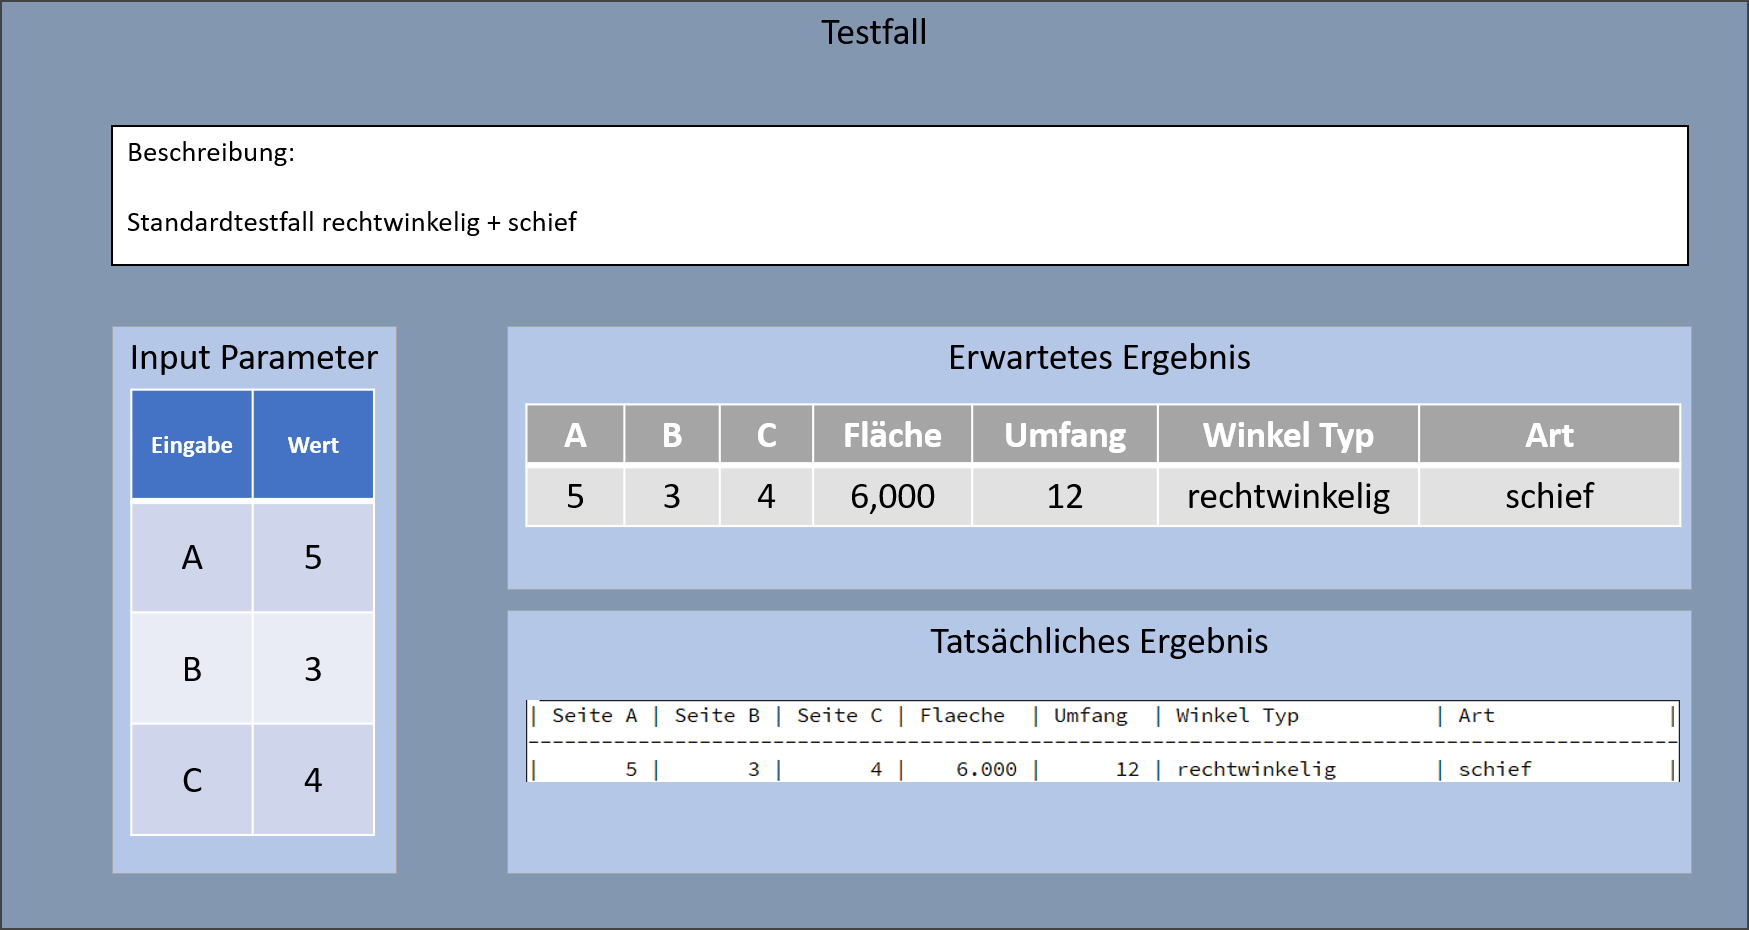
\includegraphics[width=\linewidth]{images/Testfall1.png}
    \caption{Testfall 1}
\end{figure}

\begin{figure}
    \centering
    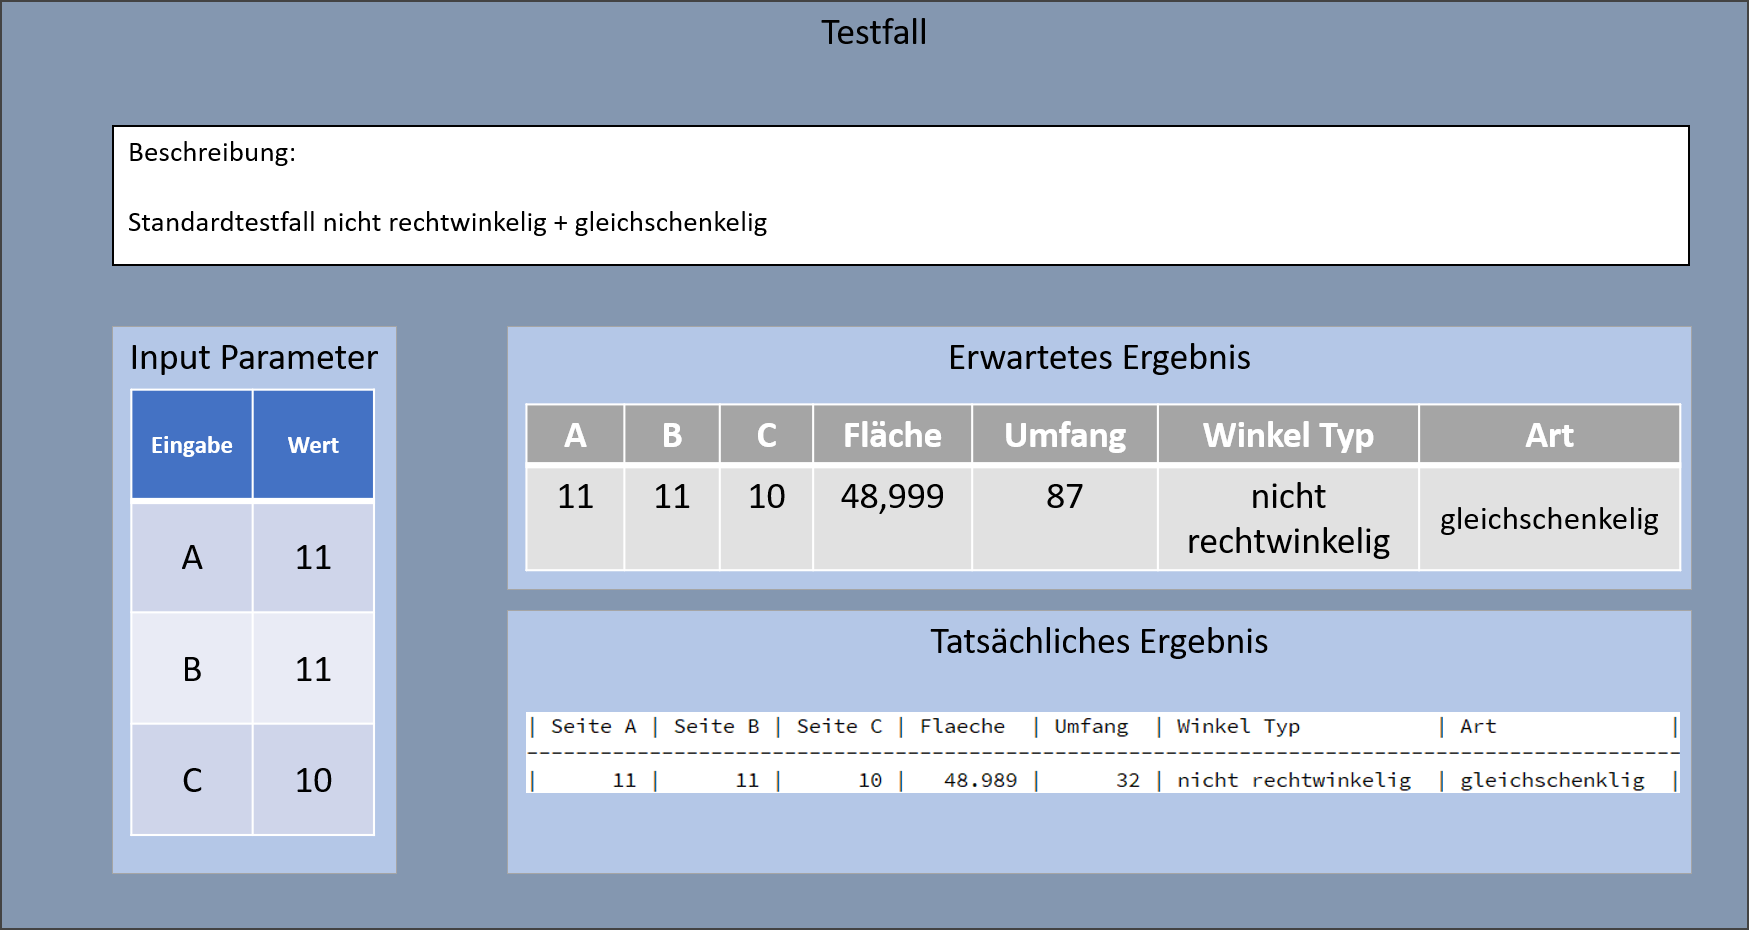
\includegraphics[width=\linewidth]{images/Testfall2.png}
    \caption{Testfall 2}
\end{figure}

\begin{figure}
    \centering
    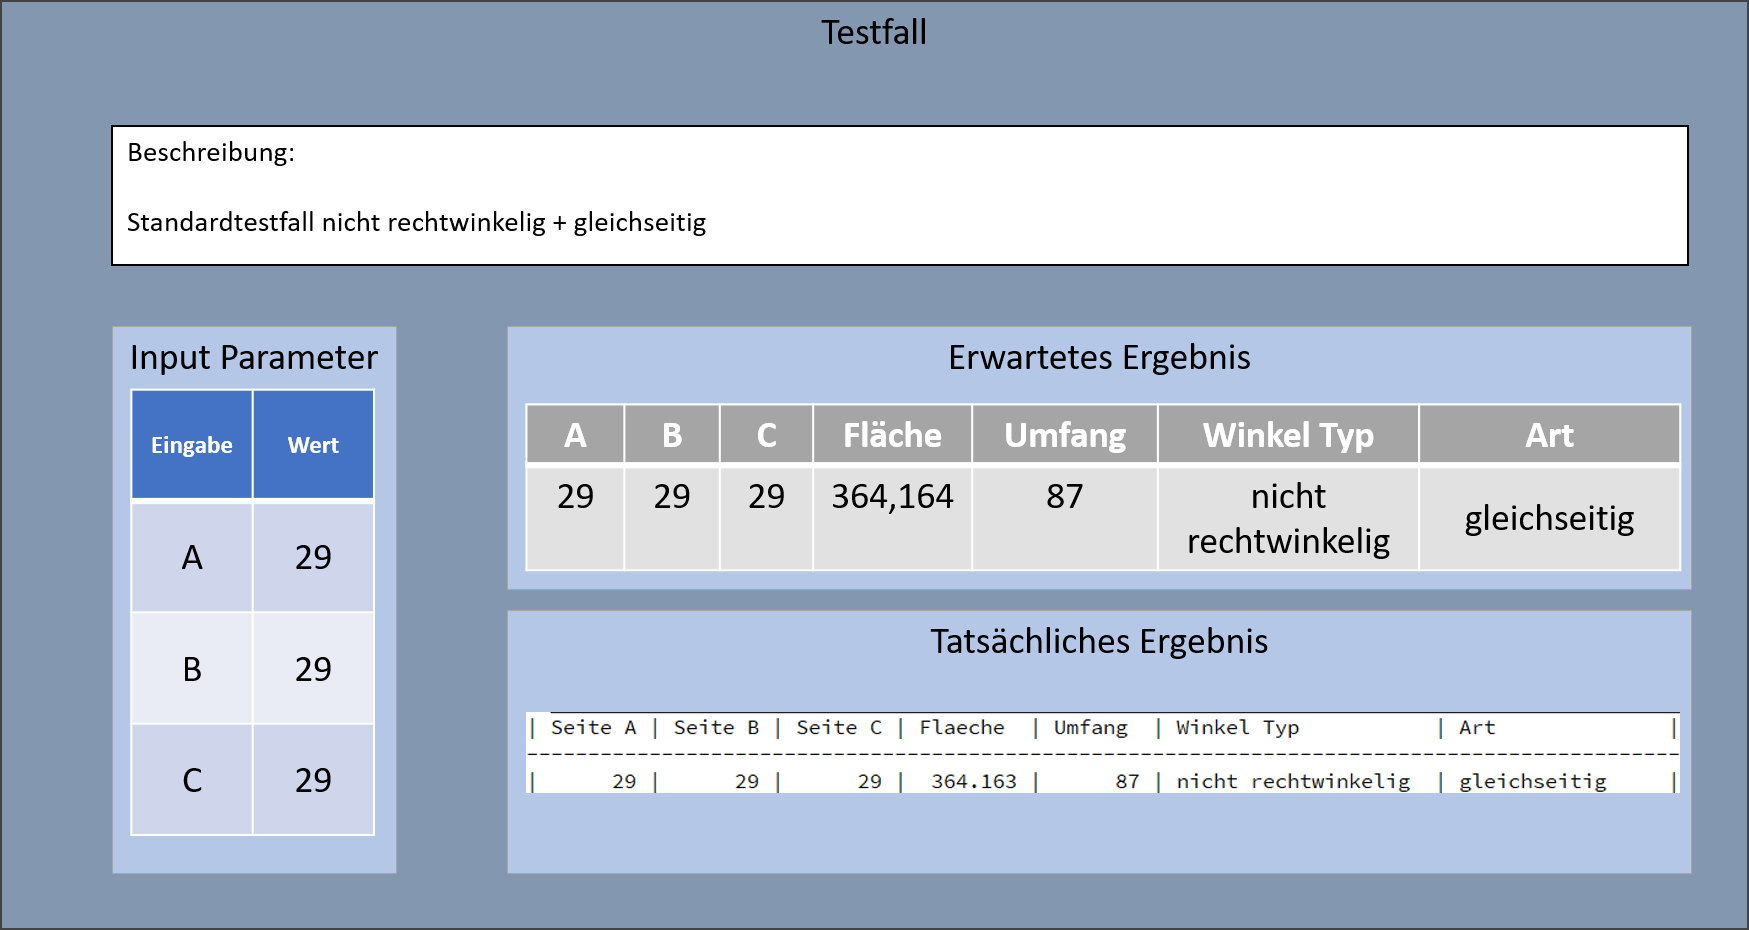
\includegraphics[width=\linewidth]{images/Testfall3.png}
    \caption{Testfall 3}
\end{figure}

\section{Ergänzende Tests}\label{sec:ergänzende_tests}

\begin{figure}
    \centering
    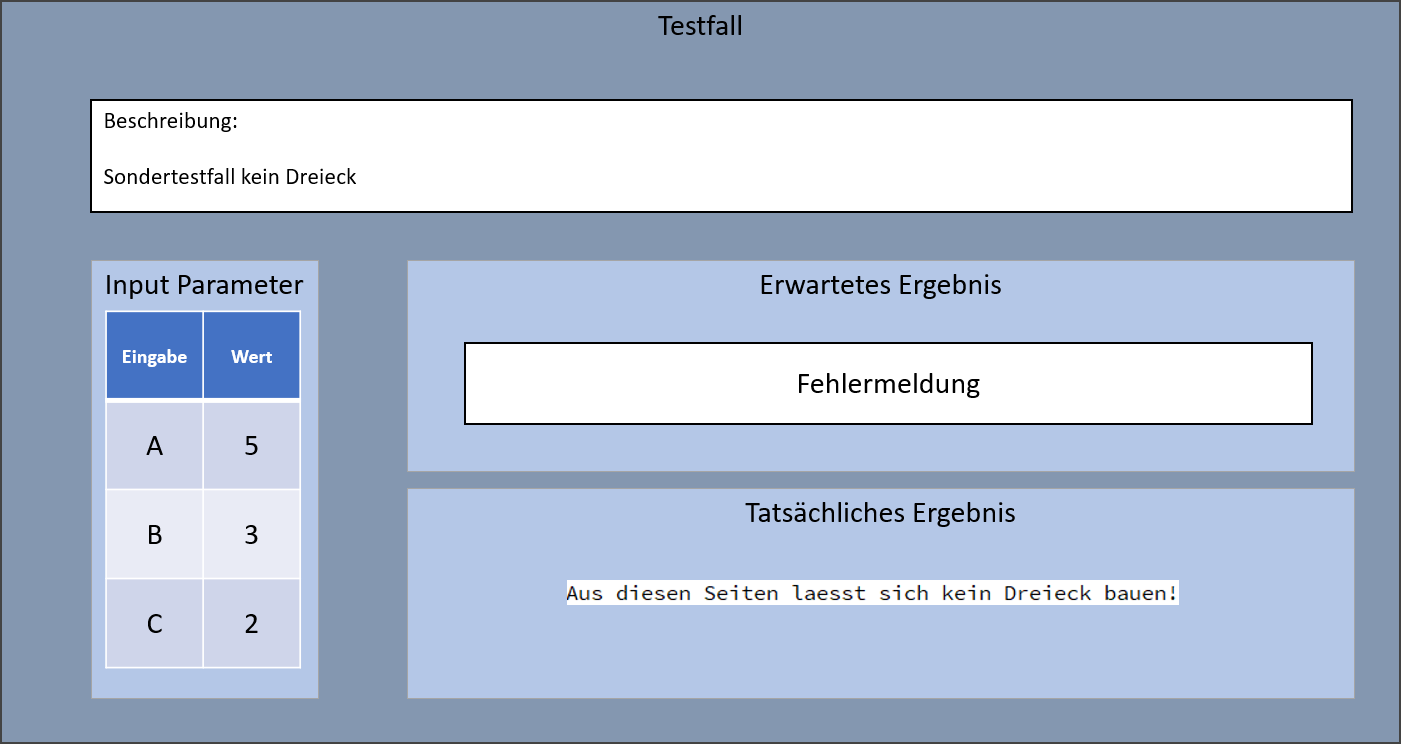
\includegraphics[width=\linewidth]{images/Testfall4.png}
    \caption{Testfall 4}
\end{figure}

\begin{figure}
    \centering
    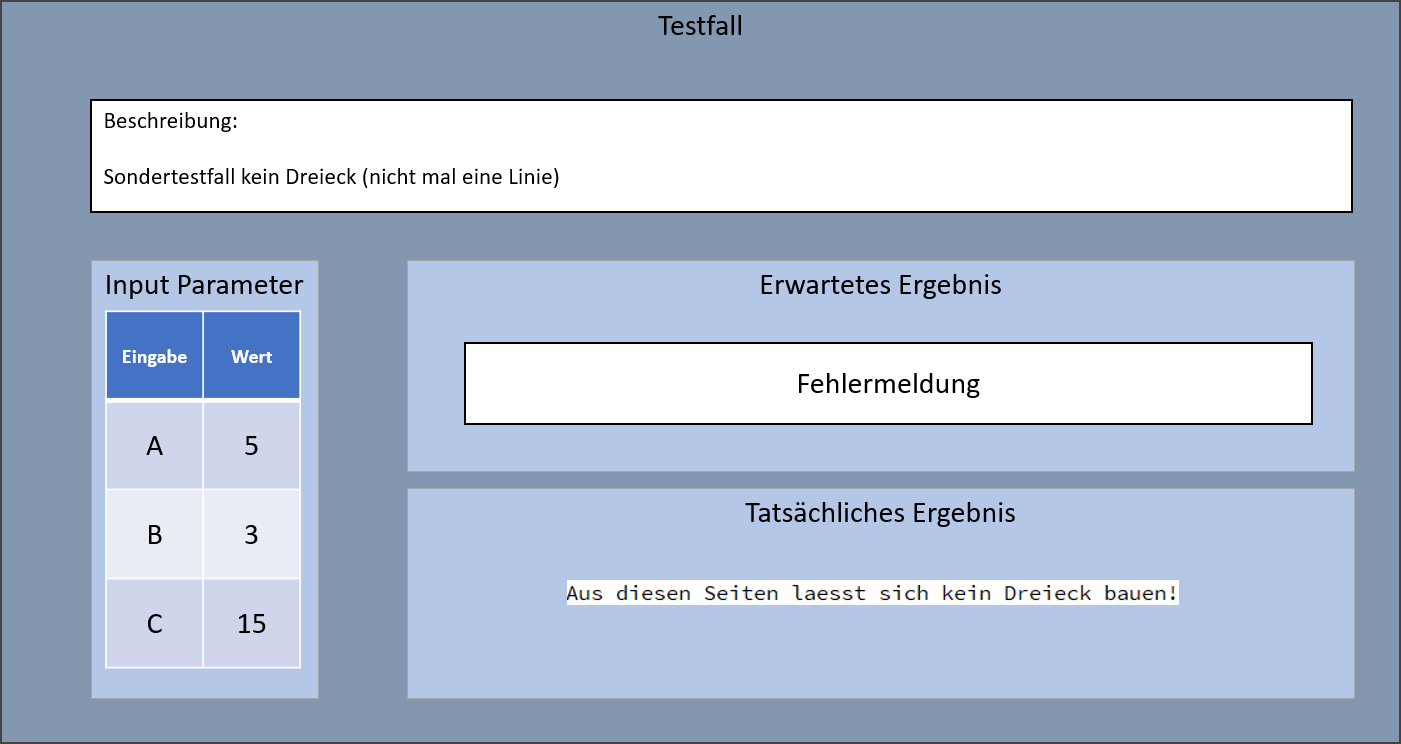
\includegraphics[width=\linewidth]{images/Testfall5.png}
    \caption{Testfall 5}
\end{figure}

\begin{figure}
    \centering
    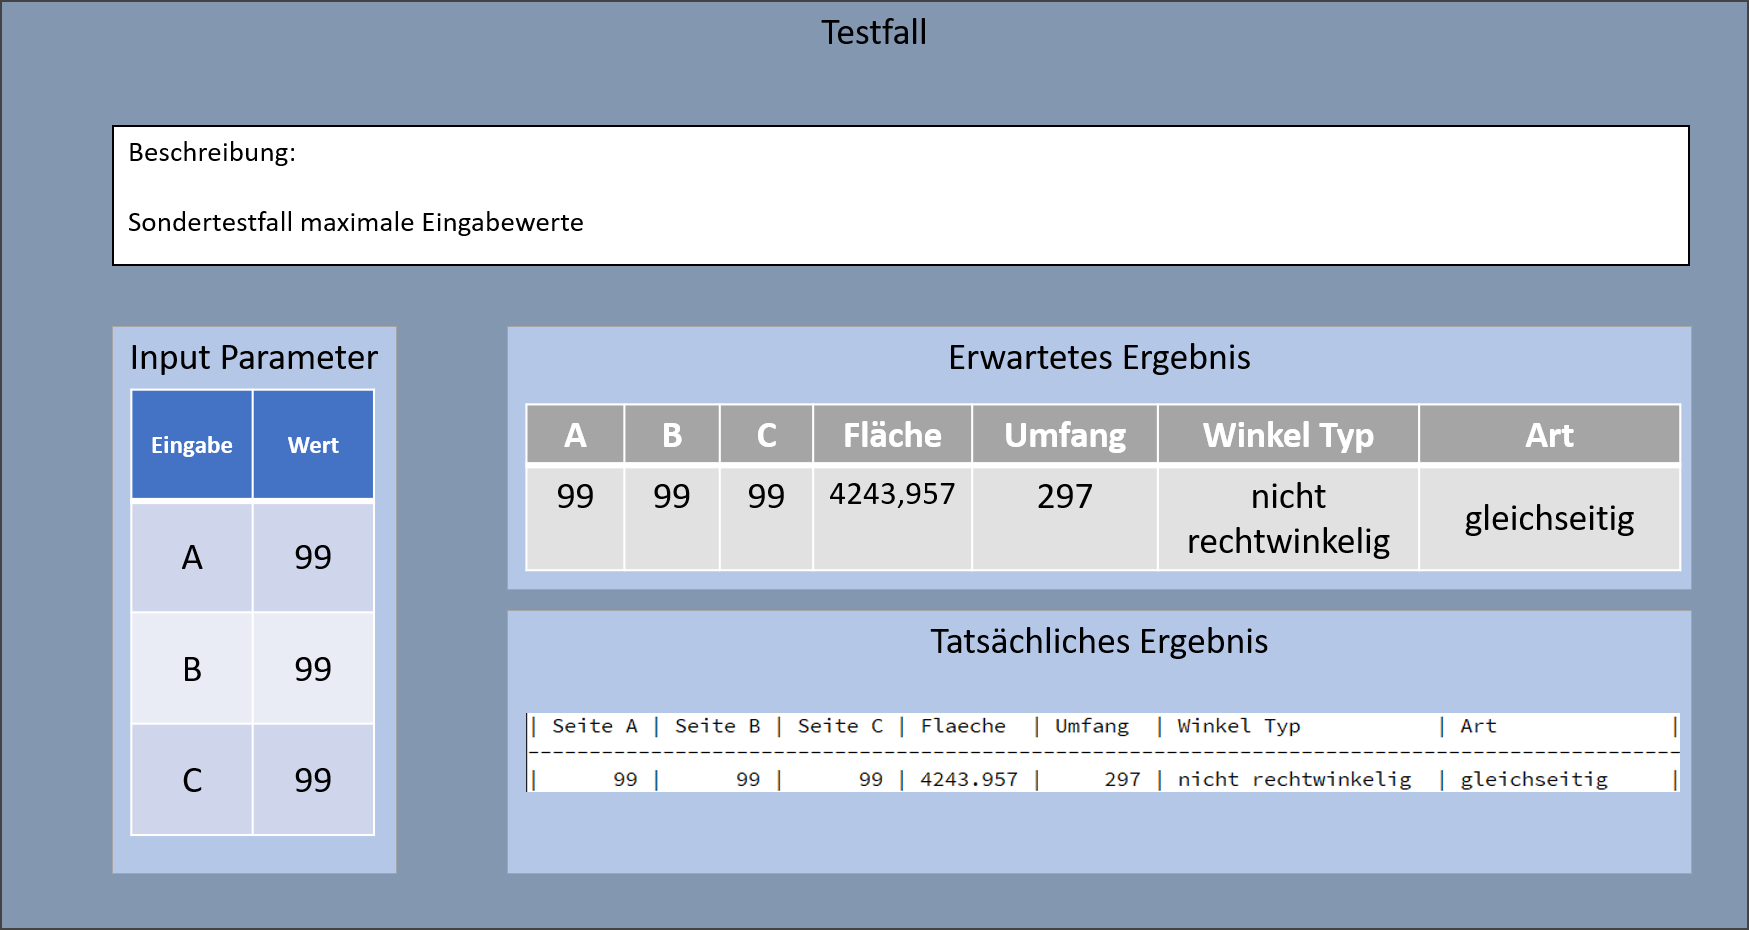
\includegraphics[width=\linewidth]{images/Testfall6.png}
    \caption{Testfall 6}
\end{figure}
\begin{figure}

    \centering
    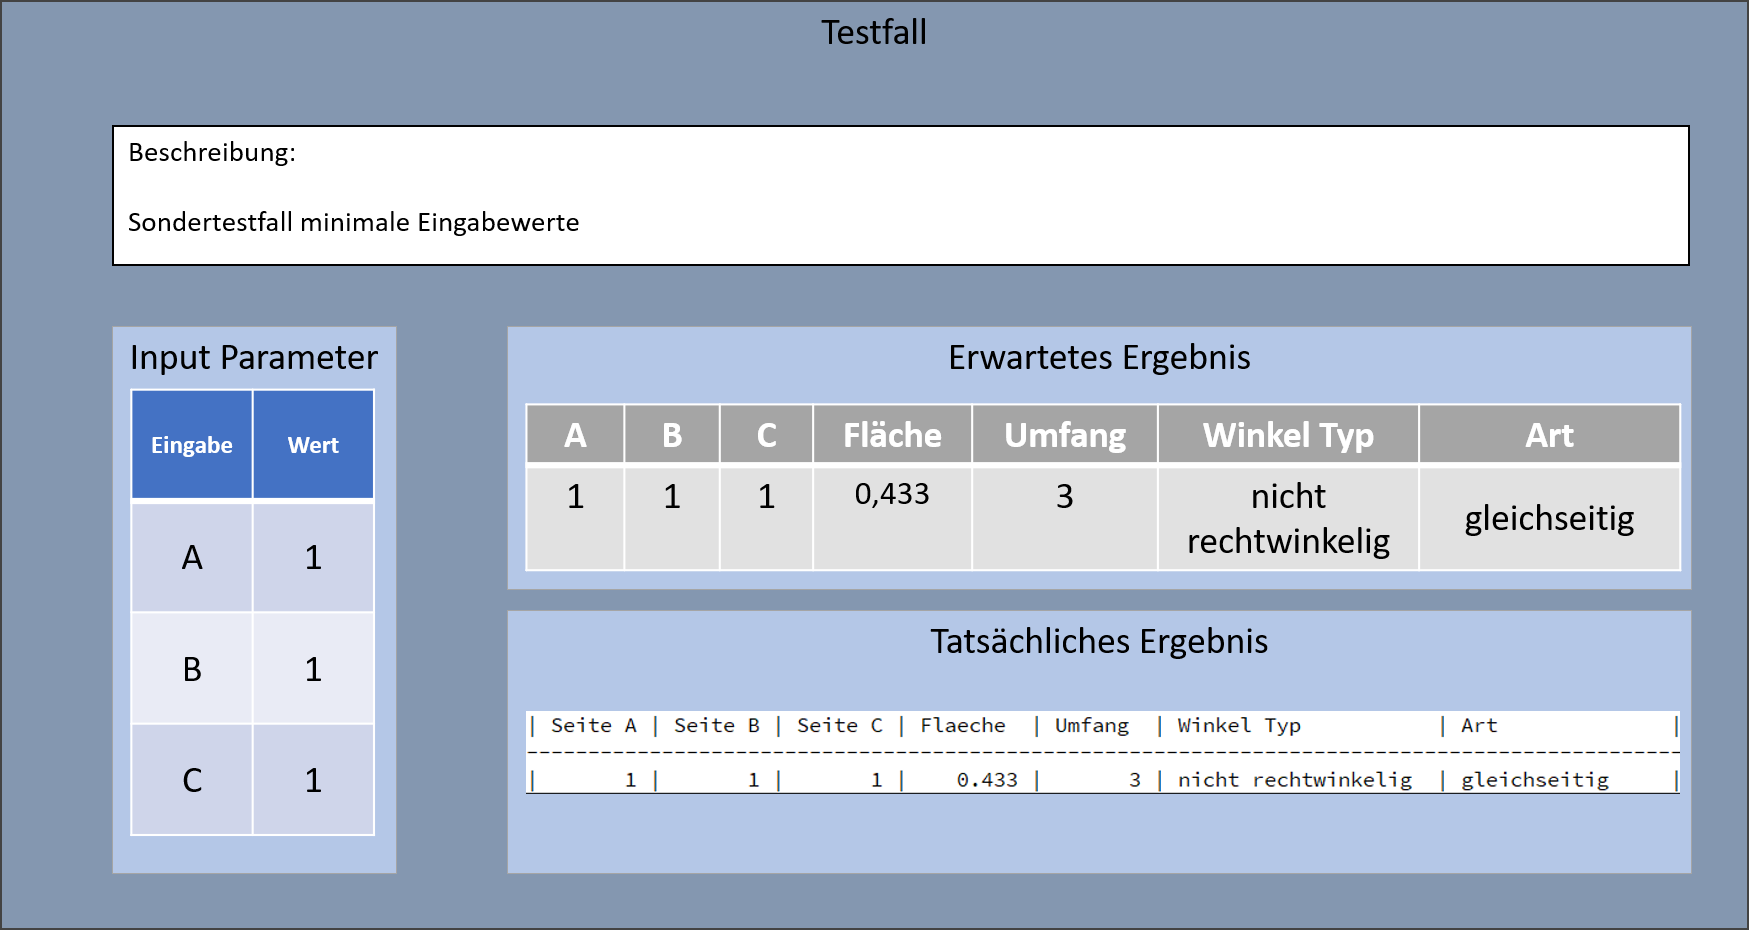
\includegraphics[width=\linewidth]{images/Testfall7.png}
    \caption{Testfall 7}
\end{figure}